\documentclass[11pt,a4paper]{article}

\usepackage[utf8]{inputenc}
\usepackage[T1]{fontenc}
\usepackage{mathpazo}
\usepackage[scaled=0.92]{helvet}
\usepackage[margin=1in]{geometry}
\usepackage{graphicx}
\usepackage{amsmath,amssymb,amsfonts}
\usepackage{booktabs}
\usepackage{tabularx}
\usepackage{setspace}
\usepackage{titlesec}
\usepackage{fancyhdr}
\usepackage{float}
\usepackage{caption}
\usepackage{microtype}
\usepackage{tikz}
\usepackage{xcolor}
\usepackage{listings}
\usepackage[hidelinks]{hyperref}

\usetikzlibrary{shapes.geometric, arrows.meta, positioning, calc, matrix, fit, backgrounds}

\setstretch{1.15}
\setlength{\parindent}{0pt}
\setlength{\parskip}{0.8em}
\sloppy

\titleformat{\section}{\normalfont\large\bfseries\sffamily}{\thesection}{1em}{}
\titleformat{\subsection}{\normalfont\normalsize\bfseries\sffamily}{\thesubsection}{1em}{}
\titleformat{\subsubsection}{\normalfont\normalsize\itshape\sffamily}{\thesubsubsection}{1em}{}

\pagestyle{fancy}
\fancyhf{}
\fancyhead[L]{\small\sffamily Stakeholder dan Aktivitas RE}
\fancyhead[R]{\small\sffamily\thepage}
\renewcommand{\headrulewidth}{0.4pt}

\captionsetup{font=small,labelfont=bf,labelsep=period}

\renewenvironment{abstract}
{\small
	\begin{center}\textbf{\sffamily Abstrak}\end{center}
	\begin{quote}}
	{\end{quote}}

\lstdefinestyle{code}{
	basicstyle=\ttfamily\small,
	frame=single,
	rulecolor=\color{black},
	breaklines=true,
	showstringspaces=false,
	columns=fullflexible,
	keepspaces=true,
	framesep=6pt,
	aboveskip=1em,
	belowskip=1em,
	xleftmargin=0pt
}

\lstdefinestyle{out}{
	basicstyle=\ttfamily\small,
	frame=tb,
	rulecolor=\color{black},
	breaklines=true,
	showstringspaces=false,
	columns=fullflexible,
	keepspaces=true,
	framesep=4pt,
	aboveskip=1em,
	belowskip=1em
}

\title{\vspace{-1.5cm}\textbf{\sffamily\LARGE Memahami Stakeholder\\ dan Aktivitas Requirement Engineering}}
\author{
	\textbf{Muhammad Riduwan Khafidi} \\
	\small Program Studi Teknik Rekayasa Perangkat Lunak \\
	\small Politeknik Negeri Batam \\
	\small \texttt{4342611034@students.polibatam.ac.id}
}
\date{\small\today}

\begin{document}

\maketitle
\thispagestyle{empty}

\begin{abstract}
	Makalah ini adalah panduan minggu kedua mata kuliah Analisis dan Spesifikasi Kebutuhan Perangkat Lunak. Ia menjelaskan mengapa keterlibatan klien menentukan berhasil atau gagalnya sebuah perangkat lunak, siapa saja yang disebut stakeholder, masalah umum yang muncul dalam relasi klien dan developer, serta dua aktivitas utama requirement engineering beserta empat sub-aktivitasnya. Tujuh visualisasi dan tiga tabel menyertai penjelasan agar pembaca dapat memahami konsep tanpa menghafal. Sebuah studi kasus berisi sepuluh langkah menunjukkan artefak konkret yang harus dihasilkan pada setiap tahap, dengan contoh kasus sistem penjadwalan kuliah. Lembar rujukan cepat di akhir merangkum istilah yang wajib dikuasai sebelum pertemuan berikutnya.
\end{abstract}

\section{Pendahuluan}

\subsection{Analogi Pembuka}

Bayangkan seorang pasien masuk ke ruang dokter. Ia mengeluh demam dan pusing. Dokter yang baik akan bertanya: sudah berapa hari, apakah disertai mual, apakah ada riwayat alergi obat. Dokter yang buruk langsung menulis resep tanpa bertanya. Kalau resepnya kebetulan cocok, pasien sembuh. Kalau tidak, penyakitnya tambah parah.

Developer perangkat lunak adalah dokter itu. Klien adalah pasiennya. Requirement engineering adalah sesi tanya-jawab sebelum resep ditulis.

\subsection{Mengapa Topik Ini Penting}

Perangkat lunak dibuat untuk memenuhi kebutuhan pengguna. Kalau developer bekerja hanya berdasarkan asumsi, ia berisiko membangun solusi untuk masalah yang salah. Keterlibatan klien sejak awal bukan formalitas. Ia adalah satu-satunya cara memastikan perangkat lunak yang dibangun benar-benar dibutuhkan.

\subsection{Peta Pembahasan}

Makalah ini disusun berurutan. Bagian kedua menjelaskan mengapa keterlibatan klien tidak bisa ditawar. Bagian ketiga mendefinisikan stakeholder dan memetakannya. Bagian keempat membeberkan masalah umum relasi klien dan developer. Bagian kelima membedah dua aktivitas requirement engineering. Bagian keenam memperdalam empat sub-aktivitas development. Bagian ketujuh menyajikan studi kasus sepuluh langkah dengan sistem penjadwalan kuliah. Bagian kedelapan sampai kesepuluh merangkum perbandingan, kesalahan umum, dan lembar rujukan cepat. Bagian kesebelas menutup dengan tiga prinsip.

\section{Mengapa Keterlibatan Klien Tidak Bisa Ditawar}

Empat kenyataan berikut menjelaskan mengapa developer tidak boleh bekerja sendirian.

\textbf{Pertama, requirement tidak boleh dibuat dari asumsi developer.} Developer tidak tahu apa yang klien butuhkan kecuali klien mengatakannya.

\textbf{Kedua, tim software biasanya tidak memahami proses bisnis klien.} Mereka menguasai teknologi, tapi belum tentu paham bagaimana faktur dibuat, bagaimana stok dihitung, atau bagaimana jadwal kuliah disusun.

\textbf{Ketiga, klien paham kebutuhannya tapi belum tentu bisa menerjemahkannya ke dokumen teknis.} Klien tahu ia ingin ``laporan yang cepat'', tapi tidak tahu bahwa ``cepat'' baginya berarti tiga detik dan bagi developer berarti dua puluh detik.

\textbf{Keempat, komunikasi yang minim menghasilkan perangkat lunak yang tidak sesuai kebutuhan.} Bug sering bukan karena kode salah, tapi karena kesepakatan awal tidak pernah tercapai.

Perhatikan Gambar~\ref{fig:loop}. Ini siklus yang terus berulang ketika komunikasi tidak dibangun dengan benar.

\begin{figure}[H]
	\centering
	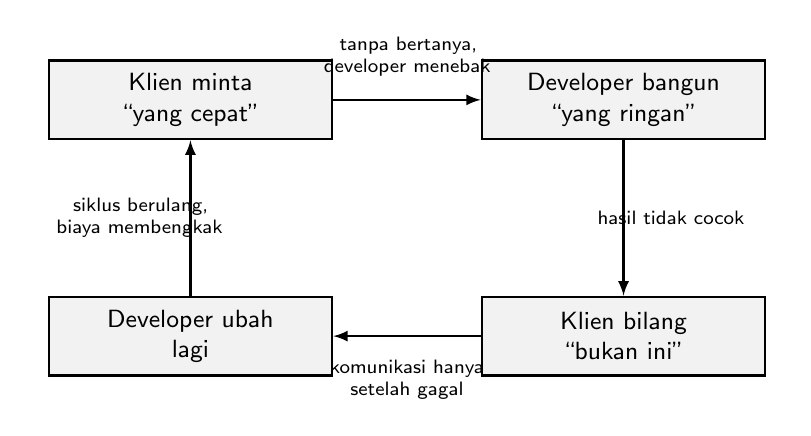
\begin{tikzpicture}[
			box/.style={rectangle, draw=black, thick, fill=black!5, minimum width=3.6cm, minimum height=1.0cm, align=center, font=\sffamily\small},
			line/.style={draw, thick, -latex},
			note/.style={font=\sffamily\scriptsize, align=center, text width=2.6cm}
		]
		\node[box] (c1) at (0, 0) {Klien minta\\``yang cepat''};
		\node[box] (d1) at (5.5, 0) {Developer bangun\\``yang ringan''};
		\node[box] (c2) at (5.5, -3) {Klien bilang\\``bukan ini''};
		\node[box] (d2) at (0, -3) {Developer ubah\\lagi};

		\draw[line] (c1.east) -- (d1.west);
		\draw[line] (d1.south) -- (c2.north);
		\draw[line] (c2.west) -- (d2.east);
		\draw[line] (d2.north) -- (c1.south);

		\node[note] at (2.75, 0.55) {tanpa bertanya,\\developer menebak};
		\node[note] at (6.1, -1.5) {hasil tidak cocok};
		\node[note] at (2.75, -3.55) {komunikasi hanya\\setelah gagal};
		\node[note] at (-0.65, -1.5) {siklus berulang,\\biaya membengkak};
	\end{tikzpicture}
	\caption{Siklus miskomunikasi yang terjadi ketika klien tidak dilibatkan sejak awal.}
	\label{fig:loop}
\end{figure}

Satu-satunya cara keluar dari siklus ini adalah memindahkan percakapan ke awal. Sebelum satu baris kode ditulis, klien dan developer harus sepakat tentang apa yang akan dibangun, mengapa dibangun, dan bagaimana mengukur keberhasilannya.

\section{Siapa Itu Stakeholder}

Stakeholder adalah individu, kelompok, organisasi, atau siapa pun yang akan terpengaruh oleh aktivitas dan keputusan dalam sebuah proyek. Kata kuncinya adalah \textbf{terpengaruh}, bukan \textbf{terlibat}. Seorang mahasiswa yang tidak pernah menyentuh sistem penjadwalan tetap stakeholder, karena jadwal kuliahnya dihasilkan oleh sistem itu.

Perhatikan Gambar~\ref{fig:stakeholder-map}. Peta ini memperlihatkan bahwa stakeholder sebuah proyek biasanya lebih banyak daripada yang diperkirakan.

\begin{figure}[H]
	\centering
	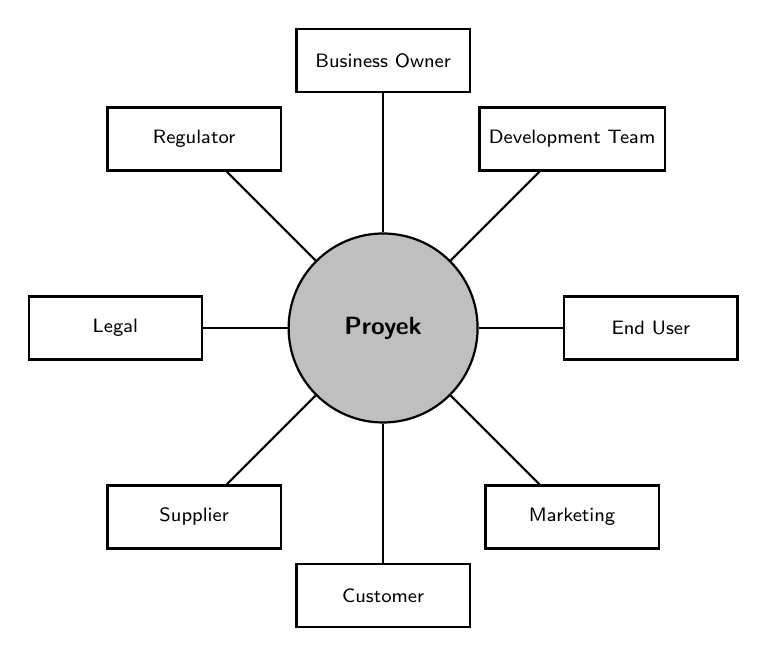
\begin{tikzpicture}[
			hub/.style={circle, draw=black, thick, fill=black!25, minimum size=2.4cm, align=center, font=\sffamily\small\bfseries},
			person/.style={rectangle, draw=black, thick, fill=white, minimum width=2.2cm, minimum height=0.8cm, align=center, font=\sffamily\scriptsize},
			line/.style={draw, thick}
		]
		\node[hub] (core) at (0,0) {Proyek};

		\node[person] (a) at (0,     3.4) {Business Owner};
		\node[person] (b) at (2.4,   2.4) {Development Team};
		\node[person] (c) at (3.4,   0)   {End User};
		\node[person] (d) at (2.4,  -2.4) {Marketing};
		\node[person] (e) at (0,    -3.4) {Customer};
		\node[person] (f) at (-2.4, -2.4) {Supplier};
		\node[person] (g) at (-3.4,  0)   {Legal};
		\node[person] (h) at (-2.4,  2.4) {Regulator};

		\draw[line] (core) -- (a);
		\draw[line] (core) -- (b);
		\draw[line] (core) -- (c);
		\draw[line] (core) -- (d);
		\draw[line] (core) -- (e);
		\draw[line] (core) -- (f);
		\draw[line] (core) -- (g);
		\draw[line] (core) -- (h);
	\end{tikzpicture}
	\caption{Peta stakeholder yang mengelilingi sebuah proyek.}
	\label{fig:stakeholder-map}
\end{figure}

Tidak semua stakeholder punya bobot yang sama. Sebagian hanya perlu diberi tahu, sebagian lain perlu dilibatkan langsung. Memetakan stakeholder berarti menentukan siapa yang masuk ke kelompok mana, dan seberapa besar pengaruhnya terhadap keputusan.

\section{Masalah Umum pada Relasi Klien dan Developer}

Tiga masalah berikut paling sering muncul. Perhatikan Gambar~\ref{fig:relation-problems}.

\begin{figure}[H]
	\centering
	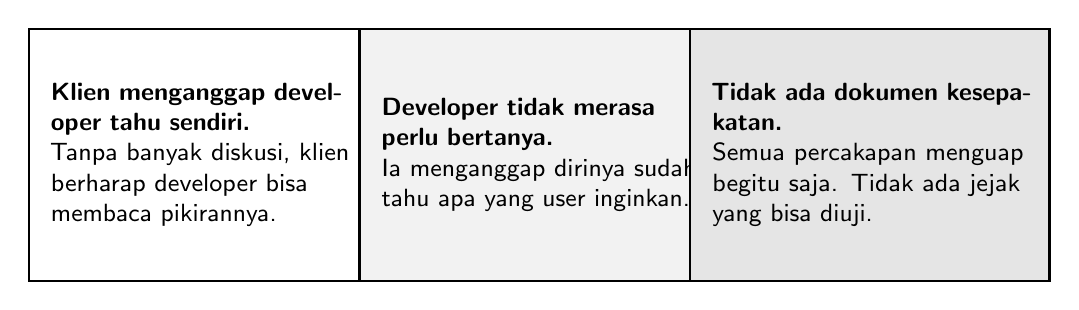
\begin{tikzpicture}[
			prob/.style={rectangle, draw=black, thick, text width=4cm, align=left, font=\sffamily\small, inner sep=8pt, minimum height=3.2cm}
		]
		\node[prob, fill=white, anchor=north west] (a) at (-6.3, 0) {
			\textbf{Klien menganggap developer tahu sendiri.} \\
			Tanpa banyak diskusi, klien berharap developer bisa membaca pikirannya.
		};
		\node[prob, fill=black!5, anchor=north west] (b) at (-2.1, 0) {
			\textbf{Developer tidak merasa perlu bertanya.} \\
			Ia menganggap dirinya sudah tahu apa yang user inginkan.
		};
		\node[prob, fill=black!10, anchor=north west] (c) at (2.1, 0) {
			\textbf{Tidak ada dokumen kesepakatan.} \\
			Semua percakapan menguap begitu saja. Tidak ada jejak yang bisa diuji.
		};
	\end{tikzpicture}
	\caption{Tiga masalah umum dalam relasi klien dan developer.}
	\label{fig:relation-problems}
\end{figure}

Perangkat lunak yang sangat baik adalah hasil dari desain yang dieksekusi dengan baik berdasarkan requirement yang sangat baik. Requirement yang sangat baik lahir dari komunikasi dan kolaborasi yang efektif antara developer dan customer. Tiga masalah di atas memutus rantai itu di titik awalnya.

\section{Dua Aktivitas Requirement Engineering}

Requirement engineering terdiri dari dua aktivitas besar. Perhatikan Gambar~\ref{fig:re-tree}.

\begin{figure}[H]
	\centering
	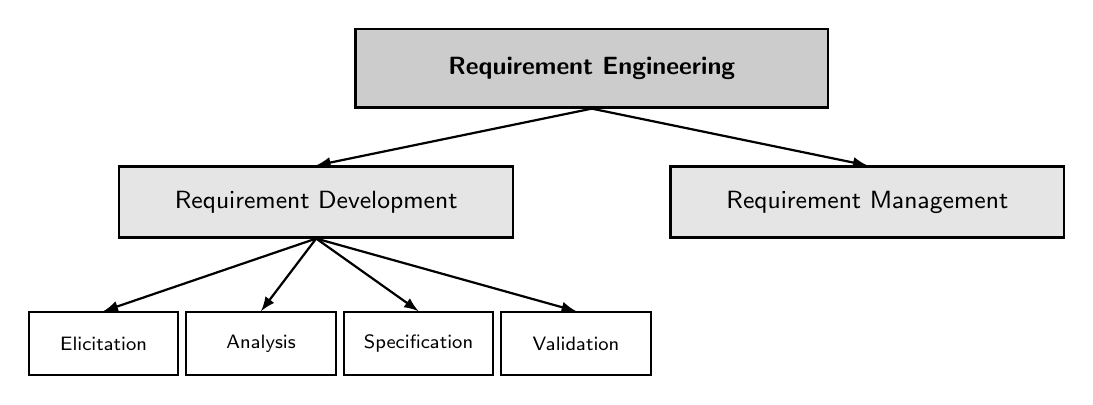
\begin{tikzpicture}[
			root/.style={rectangle, draw=black, thick, fill=black!20, minimum width=6cm, minimum height=1.0cm, align=center, font=\sffamily\small\bfseries},
			mid/.style={rectangle, draw=black, thick, fill=black!10, minimum width=5cm, minimum height=0.9cm, align=center, font=\sffamily\small},
			leaf/.style={rectangle, draw=black, thick, fill=white, minimum width=1.9cm, minimum height=0.8cm, align=center, font=\sffamily\scriptsize},
			line/.style={draw, thick, -latex}
		]
		\node[root] (eng) at (0, 4.5) {Requirement Engineering};
		\node[mid]  (dev) at (-3.5, 2.8) {Requirement Development};
		\node[mid]  (mgmt) at (3.5, 2.8) {Requirement Management};

		\node[leaf] (e) at (-6.2, 1.0) {Elicitation};
		\node[leaf] (a) at (-4.2, 1.0) {Analysis};
		\node[leaf] (s) at (-2.2, 1.0) {Specification};
		\node[leaf] (v) at (-0.2, 1.0) {Validation};

		\draw[line] (eng.south) -- (dev.north);
		\draw[line] (eng.south) -- (mgmt.north);
		\draw[line] (dev.south) -- (e.north);
		\draw[line] (dev.south) -- (a.north);
		\draw[line] (dev.south) -- (s.north);
		\draw[line] (dev.south) -- (v.north);
	\end{tikzpicture}
	\caption{Dua aktivitas utama requirement engineering dan empat sub-aktivitas development.}
	\label{fig:re-tree}
\end{figure}

\textbf{Requirement Development} mencakup semua aktivitas eksplorasi, evaluasi, dokumentasi, dan konfirmasi requirement. Ia menjawab pertanyaan: apa yang dibutuhkan.

\textbf{Requirement Management} mencakup semua aktivitas menjaga rencana proyek tetap selaras dengan requirement, melacak status dan perubahan, serta mengevaluasi dampak sebelum perubahan disetujui. Ia menjawab pertanyaan: bagaimana perubahannya dikendalikan.

Analogi sederhana: development adalah kegiatan memasak. Management adalah kegiatan mencatat bahan apa yang masuk, kapan kadaluwarsa, dan siapa yang menghabiskan. Keduanya diperlukan. Tanpa development, tidak ada makanan. Tanpa management, dapur berantakan dan bahan terbuang.

\section{Empat Sub-Aktivitas Development}

Requirement Development terdiri dari empat tahap yang berjalan berurutan. Perhatikan Gambar~\ref{fig:four-sub}.

\begin{figure}[H]
	\centering
	\begin{tikzpicture}[
			step/.style={rectangle, draw=black, thick, fill=black!5, minimum width=2.6cm, minimum height=1.4cm, align=center, font=\sffamily\small, inner sep=4pt},
			line/.style={draw, thick, -latex},
			note/.style={font=\sffamily\scriptsize, align=center, text width=2.6cm}
		]
		\node[step] (e) at (0, 0)   {Elicitation\\\scriptsize bertanya};
		\node[step] (a) at (3.4, 0) {Analysis\\\scriptsize memeriksa};
		\node[step] (s) at (6.8, 0) {Specification\\\scriptsize menuliskan};
		\node[step] (v) at (10.2, 0) {Validation\\\scriptsize mengonfirmasi};

		\draw[line] (e.east) -- (a.west);
		\draw[line] (a.east) -- (s.west);
		\draw[line] (s.east) -- (v.west);
	\end{tikzpicture}
	\caption{Empat sub-aktivitas development yang berjalan berurutan.}
	\label{fig:four-sub}
\end{figure}

\textbf{Elicitation} adalah kegiatan menggali kebutuhan. Tekniknya bisa wawancara, observasi langsung, workshop, kuesioner, atau analisis dokumen. Intinya satu: bertanya kepada stakeholder, bukan menebak.

\textbf{Analysis} adalah kegiatan memeriksa hasil elicitation. Apakah ada yang bertentangan? Apakah ada yang belum jelas? Apakah ada kebutuhan yang saling meniadakan? Analisis mencari benang merah dan konflik.

\textbf{Specification} adalah kegiatan menuliskan hasil analisis ke dalam dokumen. Requirement yang masih berupa percakapan diubah menjadi kalimat yang bisa diuji, dengan format role-goal-benefit atau input-proses-output.

\textbf{Validation} adalah kegiatan mengonfirmasi dokumen kepada stakeholder. Apakah dokumen ini benar mencerminkan kebutuhan? Apakah ada yang kurang, lebih, atau salah tafsir?

Hubungan keempatnya seperti alur memasak: belanja bahan (elicitation), periksa bahan (analysis), tulis resep (specification), sajikan untuk dicicip (validation). Kalau salah satu dilewatkan, hasilnya bisa hambar atau basi.

\section{Studi Kasus: Sistem Penjadwalan Kuliah}

Bagian ini memandu langkah demi langkah untuk menghasilkan deliverable minggu kedua. Kasus yang dipakai: sistem penjadwalan kuliah kampus. Tujuannya mengotomasi proses penyusunan jadwal yang sebelumnya dilakukan manual oleh staf akademik.

\subsection{Langkah 1: Tulis Deskripsi Singkat Sistem}

Sebelum apa pun, tulis satu paragraf tentang apa yang sistem akan lakukan.

\begin{lstlisting}[style=out]
Deskripsi Sistem:
Sistem Penjadwalan Kuliah adalah aplikasi yang
mengotomasi proses penyusunan jadwal mata kuliah
berdasarkan ketersediaan dosen, ketersediaan ruang,
dan preferensi waktu dosen. Output-nya berupa jadwal
lengkap per semester yang bisa dilihat mahasiswa,
dosen, dan staf akademik.
\end{lstlisting}

\subsection{Langkah 2: Identifikasi Stakeholder Internal}

Stakeholder internal adalah mereka yang berada di dalam tim pengembangan atau organisasi yang membangun.

\begin{lstlisting}[style=out]
Stakeholder Internal:
1. Project Manager   - mengatur waktu dan sumber daya
2. Developer Team    - membangun dan menguji sistem
3. Business Analyst  - menggali dan mendokumentasikan
4. Project Owner     - pemilik anggaran dan keputusan
\end{lstlisting}

\subsection{Langkah 3: Identifikasi Stakeholder External}

Stakeholder external adalah mereka yang berada di luar tim pengembangan tapi terpengaruh hasilnya.

\begin{lstlisting}[style=out]
Stakeholder External:
1. Staffs (staf akademik) - pengguna harian sistem
2. Lecturers (dosen)      - pemasok data preferensi
3. Students (mahasiswa)   - penerima hasil jadwal
\end{lstlisting}

\subsection{Langkah 4: Petakan Stakeholder pada Kuadran}

Tidak semua stakeholder punya bobot sama. Gunakan dua sumbu: seberapa besar pengaruh mereka terhadap keputusan, dan seberapa besar dampak keputusan pada mereka.

\begin{lstlisting}[style=out]
Kuadran Stakeholder:

Power tinggi + Interest tinggi (Manage Closely):
- Project Owner
- Staffs (staf akademik)

Power tinggi + Interest rendah (Keep Satisfied):
- Project Manager

Power rendah + Interest tinggi (Keep Informed):
- Lecturers
- Students

Power rendah + Interest rendah (Monitor):
- Tim IT pendukung
\end{lstlisting}

\subsection{Langkah 5: Tandai User Class yang Favored}

Dari daftar stakeholder external, mana yang paling kritis bagi keberhasilan produk?

\begin{lstlisting}[style=out]
User Class (Favored):
- Staffs (favored) - memakai sistem tiap hari saat
  menyusun jadwal, jika sistem gagal mereka yang
  pertama kena imbas

User Class (Supporting):
- Lecturers - mengisi data preferensi tiap awal
  semester
- Students - hanya melihat hasil jadwal
\end{lstlisting}

\subsection{Langkah 6: Rencanakan Elicitation}

Buat rencana konkret: siapa yang akan ditanya, kapan, dan dengan teknik apa.

\begin{lstlisting}[style=out]
Rencana Elicitation:

1. Wawancara dengan Project Owner (1 jam)
   Topik: visi, batasan anggaran, target waktu rilis

2. Wawancara dengan Kepala Staf Akademik (2 jam)
   Topik: alur kerja penjadwalan saat ini, kendala,
   keluhan yang sering muncul

3. Observasi langsung di ruang staf akademik (1 hari)
   Topik: melihat langsung bagaimana jadwal disusun
   manual, dokumen apa saja yang dipakai

4. Kuesioner singkat ke 30 dosen
   Topik: preferensi waktu mengajar, konflik jadwal
   yang paling sering dialami
\end{lstlisting}

\subsection{Langkah 7: Analisis Hasil Elicitation}

Setelah data terkumpul, periksa apakah ada konflik atau kesenjangan.

\begin{lstlisting}[style=out]
Temuan Analisis:

- Kebutuhan staf akademik: jadwal tidak boleh bentrok
  ruang maupun dosen
- Kebutuhan dosen: bisa memilih preferensi waktu,
  minimal dua slot per mata kuliah
- Kebutuhan mahasiswa: jadwal bisa diakses online
  sebelum semester dimulai

Konflik yang ditemukan:
- Staf ingin jadwal selesai cepat, dosen ingin
  preferensi dihormati. Sistem harus menyeimbangkan
  dua kepentingan ini.

Kesenjangan:
- Belum ada keputusan tentang siapa yang berwenang
  mengubah jadwal setelah dipublikasikan.
\end{lstlisting}

\subsection{Langkah 8: Tulis Spesifikasi Requirement}

Ubah temuan analisis menjadi requirement yang bisa diuji.

\begin{lstlisting}[style=out]
Functional Requirement:

FR-01: Sistem menghasilkan jadwal tanpa bentrok
ruang dan dosen.
Input: data mata kuliah, data dosen, data ruang.
Output: jadwal per semester yang bebas bentrok.

FR-02: Sistem menerima preferensi waktu dari dosen.
Input: slot waktu yang dipilih dosen.
Output: jadwal dengan preferensi dosen dipenuhi
sebisa mungkin.

Non-Functional Requirement:

NFR-01: Sistem menghasilkan jadwal lengkap untuk
satu semester dalam waktu kurang dari 5 menit.

NFR-02: Jadwal bisa diakses mahasiswa lewat browser
tanpa login.
\end{lstlisting}

\subsection{Langkah 9: Validasi ke Stakeholder}

Sebelum masuk pengembangan, konfirmasi dokumen ke stakeholder.

\begin{lstlisting}[style=out]
Agenda Validasi:
1. Presentasi dokumen requirement ke Project Owner
2. Review alur kerja dengan Kepala Staf Akademik
3. Uji coba prototipe jadwal dengan 5 dosen
4. Catat semua masukan, putuskan mana yang masuk
   iterasi pertama, mana yang ditunda

Kriteria Validasi:
- Semua stakeholder favored setuju isi dokumen
- Tidak ada requirement yang saling bertentangan
- Setiap requirement bisa diuji dengan data nyata
\end{lstlisting}

\subsection{Langkah 10: Tetapkan Proses Perubahan}

Setelah dokumen disahkan, tetapkan bagaimana perubahan dikelola.

\begin{lstlisting}[style=out]
Proses Change Management:

1. Setiap usulan perubahan ditulis di form change
   request berisi: deskripsi, alasan, dampak ke
   jadwal dan anggaran
2. Business Analyst mengevaluasi dampak
3. Project Owner memutuskan terima atau tolak
4. Jika diterima, dokumen requirement diperbarui
   dan versi baru diterbitkan
5. Semua perubahan dicatat di change log

Aturan:
- Tidak ada perubahan yang dikerjakan tanpa
  persetujuan Project Owner
- Setiap perubahan harus tercatat, tidak boleh lisan
\end{lstlisting}

Sepuluh langkah di atas menghasilkan tiga artefak siap kumpul: peta stakeholder, dokumen requirement hasil elicitation dan analisis, serta catatan validasi dan proses perubahan. Inilah deliverable minggu kedua.

\section{Perbandingan Ringkasan}

Tabel~\ref{tab:summary} merangkum perbedaan kunci yang telah dibahas.

\begin{table}[H]
	\centering
	\caption{Ringkasan konsep utama minggu kedua.}
	\label{tab:summary}
	\footnotesize
	\begin{tabularx}{\textwidth}{l X X}
		\toprule
		Aspek              & Konsep Pertama                  & Konsep Kedua                 \\
		\midrule
		Lokasi stakeholder & Internal (dalam tim/organisasi) & External (di luar tim)       \\
		Bobot stakeholder  & Pengaruh terhadap keputusan     & Dampak keputusan pada mereka \\
		Aktivitas RE       & Development                     & Management                   \\
		Sub-aktivitas dev  & Elicitation dan analysis        & Specification dan validation \\
		Fokus aktivitas    & Menggali dan memahami           & Mengendalikan perubahan      \\
		User class         & Favored (kritis)                & Supporting (pendukung)       \\
		\bottomrule
	\end{tabularx}
\end{table}

\section{Kesalahan Umum}

Tabel~\ref{tab:mistakes} merangkum kesalahan yang paling sering muncul saat mengerjakan tugas minggu kedua.

\begin{table}[H]
	\centering
	\caption{Kesalahan umum pada pekerjaan stakeholder minggu kedua.}
	\label{tab:mistakes}
	\footnotesize
	\begin{tabularx}{\textwidth}{l X X}
		\toprule
		Kesalahan                                         & Akibat                                    & Perbaikan                                                      \\
		\midrule
		Hanya mendaftar stakeholder tanpa memetakan bobot & Semua dianggap sama penting               & Buat kuadran power-interest                                    \\
		Menganggap semua end user identik                 & Kebutuhan satu kelas terabaikan           & Definisikan user class berdasarkan frekuensi dan kemampuan     \\
		Elicitation hanya lewat satu wawancara            & Gambaran kebutuhan tidak lengkap          & Gabungkan minimal tiga teknik: wawancara, observasi, kuesioner \\
		Tidak mencatat hasil elicitation                  & Insight hilang, tidak bisa diaudit        & Selalu tulis catatan lapangan dan transkrip singkat            \\
		Langsung menulis spesifikasi tanpa analisis       & Requirement bertentangan lolos ke dokumen & Lakukan analisis konflik dan kesenjangan sebelum menulis       \\
		Menganggap validasi selesai setelah presentasi    & Stakeholder belum benar-benar setuju      & Minta tanda tangan atau persetujuan tertulis                   \\
		Tidak menetapkan proses change management         & Requirement berubah tanpa jejak           & Tetapkan form change request dan persetujuan sponsor           \\
		Menunda dokumentasi sampai akhir                  & Semua percakapan menguap                  & Dokumentasikan sambil elicitation berlangsung                  \\
		\bottomrule
	\end{tabularx}
\end{table}

Dua kesalahan yang paling sering muncul adalah \textbf{hanya mendaftar stakeholder tanpa memetakan bobot} dan \textbf{menganggap elicitation selesai setelah satu wawancara}. Keduanya berakar pada ketergesaan yang sama: ingin cepat sampai ke pengembangan, padahal fondasinya belum kokoh.

\section{Lembar Rujukan Cepat}

Tabel~\ref{tab:cheat} adalah ringkasan istilah dan artefak yang wajib dikuasai sebelum pertemuan ketiga.

\begin{table}[H]
	\centering
	\caption{Lembar rujukan cepat untuk minggu kedua.}
	\label{tab:cheat}
	\footnotesize
	\begin{tabularx}{\textwidth}{l X}
		\toprule
		Kebutuhan atau Istilah  & Definisi atau Artefak                                                           \\
		\midrule
		Stakeholder             & Siapa pun yang terpengaruh aktivitas dan keputusan proyek                       \\
		Stakeholder internal    & Berada di dalam tim pengembangan atau organisasi                                \\
		Stakeholder external    & Berada di luar tim, tapi menerima dampak keputusan                              \\
		Stakeholder map         & Diagram yang memetakan stakeholder dan hubungannya dengan proyek                \\
		Kuadran power-interest  & Alat bantu menentukan seberapa sering stakeholder perlu dilibatkan              \\
		User class              & Kelompok pengguna berdasarkan frekuensi, kemampuan, dan hak akses               \\
		User class favored      & Kelas pengguna yang paling kritis bagi keberhasilan produk                      \\
		User class supporting   & Kelas pengguna pendukung yang tetap perlu dipenuhi kebutuhannya                 \\
		Requirement development & Aktivitas eksplorasi, evaluasi, dokumentasi, konfirmasi requirement             \\
		Requirement management  & Aktivitas tracking status, change control, evaluasi dampak perubahan            \\
		Elicitation             & Menggali kebutuhan lewat wawancara, observasi, kuesioner, atau analisis dokumen \\
		Analysis                & Memeriksa hasil elicitation: konflik, kesenjangan, konsistensi                  \\
		Specification           & Menuliskan requirement dalam bentuk yang bisa diuji                             \\
		Validation              & Mengonfirmasi dokumen requirement ke stakeholder                                \\
		Change request          & Formulir usulan perubahan requirement                                           \\
		Change log              & Catatan semua perubahan yang terjadi pada dokumen requirement                   \\
		\bottomrule
	\end{tabularx}
\end{table}

\section{Kesimpulan}

Stakeholder adalah siapa pun yang terpengaruh keputusan proyek, bukan hanya yang terlibat langsung. Memahami stakeholder berarti memetakan siapa mereka, seberapa besar pengaruh mereka, dan bagaimana mereka perlu dilibatkan. Requirement engineering terdiri dari dua aktivitas besar, development dan management, dengan empat sub-aktivitas development: elicitation, analysis, specification, dan validation. Tiga prinsip penutup:

\begin{enumerate}
	\item \textbf{Libatkan, jangan asumsikan.} Setiap stakeholder yang terpengaruh keputusan berhak menyuarakan kebutuhannya. Developer tidak boleh mengisi kekosongan itu dengan tebakan.
	\item \textbf{Petakan sebelum bertanya.} Sebelum wawancara dimulai, tentukan dulu siapa yang masuk kuadran mana. Waktu wawancara terbatas, jadi utamakan mereka yang pengaruh dan dampaknya paling besar.
	\item \textbf{Dokumentasikan sambil berjalan.} Catatan lapangan yang ditulis saat wawancara berlangsung lebih jujur daripada rangkuman yang ditulis seminggu kemudian. Ingatan menguap, dokumen tetap.
\end{enumerate}

Pada pertemuan berikutnya, prinsip-prinsip ini akan dipakai untuk mempelajari peran Business Analyst secara lebih mendalam. Lembar rujukan cepat di atas adalah bekal minimum yang harus dibawa.

\newpage
\section*{Referensi}
\addcontentsline{toc}{section}{Referensi}

\begin{thebibliography}{99}

	\bibitem{sommerville}
	Sommerville, I. (2016).
	\textit{Software Engineering} (10th ed.).
	Pearson.

	\bibitem{wiegers}
	Wiegers, K., \& Beatty, J. (2013).
	\textit{Software Requirements} (3rd ed.).
	Microsoft Press.

	\bibitem{robertson}
	Robertson, S., \& Robertson, J. (2012).
	\textit{Mastering the Requirements Process: Getting Requirements Right} (3rd ed.).
	Addison-Wesley.

	\bibitem{iiba}
	International Institute of Business Analysis. (2015).
	\textit{A Guide to the Business Analysis Body of Knowledge (BABOK Guide)} (v3.0).
	IIBA.

	\bibitem{pressman}
	Pressman, R. S., \& Maxim, B. R. (2020).
	\textit{Software Engineering: A Practitioner's Approach} (9th ed.).
	McGraw-Hill Education.

	\bibitem{cockburn}
	Cockburn, A. (2000).
	\textit{Writing Effective Use Cases}.
	Addison-Wesley.

\end{thebibliography}

\end{document}
